% ICMLDE 2026 submission
% Based on the Procedia Computer Science CRC template (Elsevier ecrc.sty)
\documentclass[3p,times,procedia]{elsarticle}
\flushbottom

\usepackage{ecrc}
\usepackage[bookmarks=false]{hyperref}
    \hypersetup{colorlinks,
      linkcolor=blue,
      citecolor=blue,
      urlcolor=blue}
\usepackage{amssymb}
\usepackage{graphicx}
\usepackage{booktabs}

\volume{00}
\firstpage{1}
\journalname{Procedia Computer Science}
\runauth{Kavinesh P et al.}
\jid{procs}

\begin{document}
\begin{frontmatter}

\dochead{International Conference on Machine Learning and Data Engineering}

\title{Why AI-Generated Image Detectors Fail on Modern Diffusion Generators: A Cross-Architecture Generalization and Failure-Mode Analysis}

\author[a]{Kavinesh P}
\author[a]{Raam Prathap R V}
\author[a]{Santhosh A S}
\author[a]{Kasam Sai Venkata Siddardha}
\author[a]{Ashish M}
\author[a]{M Anbazhagan\corref{cor1}}

\address[a]{Department of Computer Science and Engineering, Amrita School of Computing, Coimbatore 641112, Amrita Vishwa Vidyapeetham, India}

\begin{abstract}
AI-generated image detectors are usually reported as a single accuracy
number, which hides two questions that matter more for deployment: does
accuracy on one generator predict accuracy on another, and when a detector
fails, is it uncertain or confidently wrong? We evaluate five pretrained,
publicly released detectors against five generators spanning three
architecture families, with every generator verified absent from every
detector's training data. Detectors disagree about what is hard: one fails
worst on FLUX.1 (7.0\% fake-accuracy), another on SDXL (54.6\%), two others
on BigGAN (0.4\% and 9.6\%), and paired McNemar tests on identical images
confirm the gaps with a single non-significant exception between two
same-lineage detectors. Two detectors trained on identical data but
different architectures produce an \emph{identical} difficulty ordering
across all five generators ($\rho=+1.000$, exact $p=0.017$) while differing
37.6 points in mean accuracy, suggesting training data sets the shape of a
failure profile and the representation its level. Calibration error rises
with failure severity rather than falling, reaching 0.503 where
fake-accuracy is 0.4\%: these models do not degrade into uncertainty
outside their training distribution, they stay confident and become wrong.
Finally, a resize convention rarely specified in released code moves the
same checkpoint's accuracy by over 15 points, in opposite directions for
two checkpoints trained on identical data. We add two cautions: the
strongest clean-data detector on FLUX.1 falls to chance-level AUC under
ordinary JPEG re-encoding, and these benchmarks pair PNG generated images
against JPEG reals, a compression confound inflating absolute accuracy.
\end{abstract}

\begin{keyword}
AI-generated image detection \sep synthetic image forensics \sep cross-generator generalization \sep diffusion models \sep adversarial training \sep calibration \sep reproducibility
\end{keyword}
\cortext[cor1]{Corresponding author: M Anbazhagan}
\end{frontmatter}

\email{m\_anbazhagan@cb.amrita.edu}

\vspace*{-6pt}

\section{Introduction}
\label{sec:intro}

A detector's accuracy number is only useful if it predicts behavior on data
the detector has not seen. In practice, a detector trained on one
generator's outputs is regularly reported to lose most of its accuracy on a
different generator's outputs, and the field has largely explained this with
a single story: newer, more sophisticated generators produce artifacts that
older detectors were not built to catch. That story predicts a specific
pattern. Detectors should fail worst on the newest generators, and that
failure should look broadly similar across detectors that were not trained
on them.

We test the prediction by running five independently trained, publicly
released detectors against five generators spanning three architecture
families, and it does not hold. The detectors disagree about which
generator is hardest: one fails worst on FLUX.1, another on SDXL, and two
others on BigGAN, the oldest generator in the set. In the sharpest case,
one detector recovers 5{,}452 FLUX.1 images that another misses while
losing only 8 in the opposite direction, on the identical image set.
Generator age is not the variable driving detector failure; the detector's
own training distribution is.

This paper makes four contributions. We report a controlled generalization
audit of five detectors on five generators, run entirely by inference over
released checkpoints and datasets, with training/test overlap verified
against primary documentation rather than inferred from the accuracy
pattern such a check is meant to validate, and every reported gap backed by
a paired McNemar test (Section~\ref{sec:significance}). We then decompose
the disagreement: including two detectors trained on identical data but
different architectures separates the contribution of training data from
that of representation, and their difficulty orderings match exactly while
their accuracy levels differ by 37.6 points
(Section~\ref{sec:finding-shape}). We give a calibration account of the
failure mode, showing that calibration error rises together with error rate
rather than falling (Section~\ref{sec:confidence}), which is what makes a
generalization gap dangerous in deployment. Finally we report a
reproducibility finding: a 6x discrepancy against a source paper's own
number traced to a metric-definition mismatch plus a genuine preprocessing
effect, which we replicate on a second generator and decompose into a
recoverable threshold shift and an information-destroying distortion
(Section~\ref{sec:discussion}). Two related cautions follow, on JPEG
re-encoding (Section~\ref{sec:robustness}) and on a PNG-versus-JPEG
compression asymmetry in the benchmarks themselves
(Section~\ref{sec:jpeg-confound}).

\textbf{A note on terminology.} ``Deepfake'' originally named a narrower
problem: face swapping and reenactment, where the manipulated region is a
face inside an otherwise real photograph. We study the broader task of
deciding whether an entire image was synthesised, over ImageNet-style
object and scene imagery, which is more precisely called AI-generated image
detection, and that is the term we use. The two problems have different
artifact structures and largely separate literatures
(Section~\ref{sec:related}); nothing here should be read as a claim about
face-manipulation detection.

Section~\ref{sec:related} places this work against the generalization and
adversarial-training literature it builds on. Section~\ref{sec:methods}
describes the five detectors, five generators, and the leakage, threshold,
and sample-size controls applied uniformly across them.
Section~\ref{sec:results} reports the cross-detector comparison, the paired
significance tests behind it, and the calibration analysis.
Section~\ref{sec:discussion} walks through the preprocessing investigation
as a self-contained methodological case study.
Section~\ref{sec:robustness} reports a JPEG re-encoding robustness check.
Section~\ref{sec:limitations} states what this study does not establish,
Section~\ref{sec:ethics} covers dual-use considerations, and
Section~\ref{sec:conclusion} closes.

\section{Related Work}
\label{sec:related}

\textbf{Cross-generator generalization.} Wang et al.~\cite{wang2020cnndetect}
established the standard protocol of training on one GAN family (ProGAN)
and testing against unseen GANs. Zhu et al.'s GenImage~\cite{genimage2023}
extended it to diffusion models at million-image scale and is the training
source for three of the five detectors we evaluate. Ojha et al.'s
UniversalFakeDetect~\cite{ojha2023universal} showed that a frozen CLIP
embedding with a linear probe, trained only on ProGAN, transfers to GANs
and early diffusion models better than end-to-end training; we use it as
our CLIP-embedding baseline. Tan et al.'s NPR~\cite{tan2024npr} instead
targets neighbouring-pixel artifacts left by a generator's up-sampling
operations, and is the one detector here whose training data and detection
signal are both unrelated to CLIP. Other work keeps the CLIP embedding but
changes the head: C2P-CLIP~\cite{tan2025c2pclip} injects a learned category
prompt, and DIRE~\cite{wang2023dire} detects diffusion images by how well a
diffusion model reconstructs them. We evaluate neither, but both show that
the field's usual response to the generalization gap is architectural,
building a detector expected to transfer, rather than asking why a given
detector's training distribution predicts where it fails.

\textbf{The adversarial-training comparison.} Zhou et
al.~\cite{zhou2025omat} attribute cross-generator failure to \emph{latent
prior bias}: a detector can key on artifacts of its training generator's
initial-noise sampling rather than of the generation process. The
hypothesis builds on Xu et al.~\cite{xu2025seeds}, who recovered the random
seed used to sample a diffusion model's initial noise from the generated
image, showing such a shortcut exists to be learned. Their fix, On-Manifold
Adversarial Training (OMAT), fine-tunes against adversarially optimized
initial latents of the \emph{same} training-time generator, and their
GenImage++ benchmark adds held-out subsets from FLUX.1~\cite{flux2024} and
Stable Diffusion 3~\cite{esser2024sd3}, plus tests against the in-the-wild
Chameleon collection~\cite{yan2024chameleon}. We neither modify nor retrain
their checkpoints; we evaluate them alongside unrelated detectors on a
wider generator set, and additionally test whether their preprocessing
choice is load-bearing, which their evaluation did not need to ask.

\textbf{Generators, and two boundaries of scope.}
BigGAN~\cite{brock2019biggan} is a class-conditional GAN;
GLIDE~\cite{nichol2021glide} and SDXL~\cite{podell2023sdxl} are early and
modern U-Net diffusion models; FLUX.1 and SD3 replace the U-Net denoiser
with a Diffusion Transformer~\cite{peebles2023dit}. This spread is our independent
variable, grouped by architecture family rather than release date, since
our results show family predicts detector behaviour better than recency.
Two boundaries are worth stating. First, the detectors here are not
face-manipulation deepfake detectors, which target a local edit inside a
genuine photograph, and are benchmarked on face corpora such as
FaceForensics++~\cite{rossler2019ff} and Celeb-DF~\cite{li2020celebdf}; a
face-swap artifact is a local inconsistency, whereas our generators
synthesise every pixel, so the two settings do not share an artifact
model. Second, our
Section~\ref{sec:confidence} analysis of \emph{how} detectors fail sits
beside a small interpretability literature: frequency-domain
analyses~\cite{qian2020freq,frank2020leveraging} attribute behaviour to
spectral artifacts, and Grad-CAM-style
attribution~\cite{selvaraju2017gradcam} visualises which regions drive a
classifier. We take a coarser route, characterising the predicted
probability distribution and its calibration error, which answers a
different question and assumes nothing about which regions carry the
evidence. Pixel-level attribution of the confident failures we identify is
a natural follow-up we do not attempt.

\section{Methodology}
\label{sec:methods}

Every result comes from running a pretrained, publicly released detector
checkpoint over a pretrained, publicly released image dataset, with no
training and no image generation. This began as a hardware constraint,
since the single 8~GB consumer GPU used throughout cannot hold a generation
pipeline and a detector at once, but it has the useful effect of making the
pipeline reproducible without generation infrastructure.

\subsection{Detectors}

Table~\ref{tab:detectors} lists the five detectors. Three use a frozen
CLIP~\cite{radford2021clip} ViT-L/14 encoder with a linear (or
LoRA~\cite{hu2022lora}-adapted) probe; the other two are convolutional, one
keying on pixel/up-sampling artifacts and one a plain ResNet-50. Training
composition was confirmed for each detector from its own repository
documentation, and for the GenImage++ checkpoints from the source paper's
stated methodology (Section~\ref{sec:methods-leakage}), rather than
inferred from how well each performed.

The GenImage++ ResNet-50 is included for a specific reason: it was trained
on exactly the same data as the GenImage++ CLIP baseline but is a
conventional CNN with no CLIP backbone. It is therefore the one pair here
that varies architecture while holding training data fixed, which is what
lets Section~\ref{sec:finding-shape} separate what the training
distribution does from what the representation does.

\begin{table}[h]
\caption{Detectors evaluated. All five are used as released, with no
fine-tuning performed for this study.}
\label{tab:detectors}
\begin{tabular*}{\hsize}{@{\extracolsep{\fill}}p{2.15cm}p{2.6cm}p{4.3cm}p{1.5cm}@{}}
\toprule
Detector & Signal & Training data (verified) & Source \\
\colrule
UniversalFakeDetect & CLIP ViT-L/14 embedding + linear probe & ProGAN only, 20 LSUN categories & \cite{ojha2023universal} \\
NPR & Pixel / up-sampling artifact (ResNet-50) & ProGAN only, 4 LSUN categories & \cite{tan2024npr} \\
GenImage++ ResNet-50 & Plain CNN classifier (no CLIP) & GenImage SDv1.4 subset only & \cite{zhou2025omat} \\
GenImage++ CLIP & CLIP ViT-L/14 embedding + linear probe & GenImage SDv1.4 subset only & \cite{zhou2025omat} \\
GenImage++ CLIP-LoRA (OMAT) & Same backbone + LoRA, on-manifold adversarial fine-tune & Same SDv1.4 data + 6{,}000 SDv1.4-derived adversarial examples & \cite{zhou2025omat} \\
\botrule
\end{tabular*}
\end{table}

\subsection{Evaluation protocol}
\label{sec:methods-protocol}

Each detector outputs one probability that an image is generated. We
threshold at \textbf{0.5} for every accuracy figure, for every detector and
generator, with no tuning. Because a fixed threshold can flatter or
penalise a detector whose scores are shifted, we report threshold-free AUC
alongside and treat calibration separately in
Section~\ref{sec:confidence}.

We report real- and fake-accuracy separately rather than only overall
accuracy, since a degenerate detector labelling everything ``generated''
would score 100\% fake-accuracy and that column alone could not distinguish
it from genuine detection. Real-accuracy stays between 86.0\% and 98.9\%
across all 25 cells, so no detector approaches that failure mode, and the
converse case is visible rather than hidden: the GenImage++ ResNet-50 on
BigGAN sits at 98.5\% real- and 0.4\% fake-accuracy, close to labelling
everything real, and we report it as such.

For the ResNet-50 the released code and the source paper disagree on input
normalization, the former routing every detector through CLIP statistics
and the latter specifying ImageNet statistics. We measured both and used
ImageNet statistics, which performed better (85.3\% versus 80.7\%
fake-accuracy on a 150-image FLUX.1 probe): a small instance of the
under-specification problem Section~\ref{sec:discussion} treats at
length.

\subsection{Generators and evaluation data}

BigGAN and GLIDE come from the original GenImage
benchmark~\cite{genimage2023}, each evaluated against its own paired real
split rather than a shared pool. FLUX.1, SD3 and SDXL come from
GenImage++~\cite{zhou2025omat}, documented by its authors as test-only,
which ships fake images only; since it has no matched reals, we use
GenImage's BigGAN-subset real training split (about 162{,}000 ImageNet
images, disjoint from the 6{,}000 used as BigGAN's own paired real
evaluation split) as a shared real pool for all three. This asymmetry
against the BigGAN/GLIDE evaluation is forced by the dataset and we flag it
rather than leave it implicit. BigGAN is a GAN, GLIDE and SDXL are
U-Net diffusion models (early and modern respectively), and FLUX.1 and SD3
are Diffusion Transformers.

We use 6{,}000 real and 6{,}000 fake images for BigGAN, GLIDE, FLUX.1 and
SD3, and the full 18{,}300--18{,}301 per class for SDXL. At worst-case
proportions this gives a 95\% confidence-interval half-width of $\pm$1.26
points at $n=6{,}000$ against $\pm$0.72 at $n=18{,}300$; every gap we
report is tens of points, so the asymmetry changes no conclusion. One
further note affects how these sizes should be read: an early version of
our evaluation silently capped every run at 100 images per class, because
the dataset loader we inherited falls back to that default whenever the
requested size exceeds either class pool, which was always true here, so a
flag meaning ``use all available data'' had the opposite effect. Every
number here comes from full-data reruns after that was found, and we
mention it because the failure was silent and produced plausible-looking
results.

\subsection{Training/test leakage verification}
\label{sec:methods-leakage}

Because the central claim of this paper is that detectors fail to
generalize, it matters that ``fail to generalize'' is not secretly ``fail
on data it never should have seen for an unrelated reason.'' The mirror
image matters even more given how large the OMAT improvement in
Section~\ref{sec:results} is: ``succeed'' could just as easily be secretly
leakage rather than genuine generalization, and that is the more
consequential failure mode to rule out. We
checked training-data composition against primary sources rather than
inferring it from the accuracy pattern the check exists to validate.
UniversalFakeDetect and NPR both document ProGAN-only training in their own
repository READMEs, with NPR's training command explicitly restricted to
four ProGAN-generated LSUN categories and BigGAN appearing in that
repository's folder layout only under a held-out test split, never
referenced by the training command. For the GenImage++ pair, we quote the
source paper directly (Zhou et al.~\cite{zhou2025omat}, Section 6.1):
``all detectors, including our initial baselines and external methods,
were trained on the Stable Diffusion v1.4 (SDv1.4) subset of GenImage...
For adversarial training, these baseline detectors were subsequently
fine-tuned using the SDv1.4 training data augmented with $N=6{,}000$ of our
on-manifold adversarial examples,'' and the same paper's Section 3.3
confirms those 6{,}000 adversarial examples are themselves rendered from
Stable Diffusion v1.4. GenImage++'s own evaluation subsets (FLUX.1, SD3,
SDXL) are independently documented by the same paper as test-only.
None of the five generators in our evaluation set appears in any of the
five detectors' training data.

\section{Results}
\label{sec:results}

Table~\ref{tab:results} gives fake- and real-accuracy for every detector
and generator, and Table~\ref{tab:auc} gives threshold-free AUC and
calibration error for the same cells, all under each detector's officially
released preprocessing.

\begin{table}[h]
\caption{Fake-accuracy / real-accuracy (\%) at threshold 0.5. Bold marks
each detector's own worst generator by fake-accuracy. Real-accuracy is
reported alongside so the fake column cannot be read as evidence for a
detector that simply predicts ``generated'' everywhere.}
\label{tab:results}
\begin{tabular*}{\hsize}{@{\extracolsep{\fill}}lccccc@{}}
\toprule
Detector & BigGAN & GLIDE & FLUX.1 & SD3 & SDXL \\
\colrule
UniversalFakeDetect & 83.0 / 97.4 & 27.4 / 97.7 & \textbf{7.0} / 96.8 & 11.7 / 96.8 & 38.5 / 96.8 \\
NPR & 84.1 / 86.0 & 94.3 / 86.2 & 97.7 / 88.1 & 90.1 / 88.1 & \textbf{54.6} / 87.7 \\
GenImage++ ResNet-50 & \textbf{0.4} / 98.5 & 6.0 / 98.3 & 54.9 / 98.9 & 66.1 / 98.9 & 15.2 / 98.6 \\
GenImage++ CLIP & \textbf{9.6} / 96.5 & 69.1 / 96.0 & 86.5 / 97.4 & 88.6 / 97.4 & 77.0 / 97.4 \\
GenImage++ CLIP-LoRA & 99.7 / 94.8 & 99.9 / 94.9 & \textbf{96.5} / 96.0 & 98.3 / 96.0 & 99.2 / 94.7 \\
\botrule
\end{tabular*}
\end{table}

\begin{table}[h]
\caption{AUC (\%) and expected calibration error (ECE, 15 bins, lower
better) by detector and generator. AUC is threshold-free; ECE rises with
failure severity rather than falling, the signature of confident error
discussed in Section~\ref{sec:confidence}.}
\label{tab:auc}
\begin{tabular*}{\hsize}{@{\extracolsep{\fill}}lccccc@{}}
\toprule
Detector (AUC / ECE) & BigGAN & GLIDE & FLUX.1 & SD3 & SDXL \\
\colrule
UniversalFakeDetect & 98.2 / .042 & 85.6 / .300 & 61.4 / .439 & 72.5 / .406 & 85.4 / .245 \\
NPR & 91.3 / .126 & 95.2 / .084 & 96.9 / .060 & 94.4 / .091 & 76.5 / .268 \\
GenImage++ ResNet-50 & 51.4 / .503 & 60.3 / .469 & 86.2 / .212 & 92.8 / .153 & 68.8 / .415 \\
GenImage++ CLIP & 68.0 / .433 & 94.0 / .120 & 98.6 / .034 & 98.7 / .031 & 97.0 / .076 \\
GenImage++ CLIP-LoRA & 99.7 / .015 & 99.8 / .015 & 99.3 / .020 & 99.7 / .015 & 99.4 / .012 \\
\botrule
\end{tabular*}
\end{table}

\subsection{Detectors disagree on which generator is hardest}
\label{sec:finding1}

Detectors do not agree on what is hard. UniversalFakeDetect fails worst on
FLUX.1 (7.0\%), NPR on SDXL (54.6\%), and both GenImage++ non-adversarial
baselines on BigGAN (0.4\% for ResNet-50, 9.6\% for CLIP). CLIP-LoRA is
lowest on FLUX.1 too, but at 96.5\%, only 3.4 points below its own best, so
``worst generator'' is a weak label there and we treat it separately in
Section~\ref{sec:finding2}.

The clearest illustration is the GenImage++ CLIP baseline, which catches
86--89\% of FLUX.1 and SD3 fakes, the exact generators UniversalFakeDetect
almost entirely misses, while catching under 10\% of BigGAN, which
UniversalFakeDetect and NPR both catch above 82\% and CLIP-LoRA at 99.7\%.
If recency alone drove difficulty, no detector should recover on the oldest
generator what it loses on the two newest. What predicts a weak spot is
which generator family the training data did not cover, old or new.

\subsection{The gaps are statistically significant, with one informative
exception}
\label{sec:significance}

Differences read off a table are not evidence, so we test them. All five
detectors scored the \emph{identical} fake-image set for each generator
(6{,}000 images; 18{,}300 for SDXL), making the comparison paired and
admitting McNemar's test~\cite{mcnemar1947}. For detectors $A$ and $B$ we
count $n_{01}$, images $A$ gets right and $B$ does not, and $n_{10}$, the
reverse, and run an exact two-sided binomial test on the discordant pairs.
We restrict to fake images because the real-image sets are matched across
detectors only for BigGAN and GLIDE (Section~\ref{sec:limitations}).

Table~\ref{tab:mcnemar} gives the tests the argument rests on. The FLUX.1
contrast is decisive: NPR classifies 5{,}452 FLUX.1 fakes correctly that
UniversalFakeDetect misses, against 8 the other way, $p<10^{-300}$. The
same two detectors on the identical 12{,}000-image FLUX.1 set produce
5{,}864 versus 420 correct fake calls, opposite outcomes on the same
images, which is the sharpest evidence in this study that generalization
failure is a detector property rather than a property of how hard a
generator is.

The informative exception is BigGAN, where UniversalFakeDetect and NPR
score 82.95\% and 84.12\%, and it would be easy to call NPR better. The
paired test disagrees: 835 images go one way and 905 the other, $p=0.098$.
Of 50 pairwise tests (ten detector pairs across five generators) this is
the only one failing significance at $\alpha=0.05$; the next weakest still
reaches $p=9.6\times10^{-3}$. Those two detectors are indistinguishable on
BigGAN and the 1.2-point gap should not be interpreted, which strengthens
Section~\ref{sec:finding1} rather than weakening it: BigGAN is where the
two ProGAN-trained detectors behave alike, as a shared training lineage
predicts, while every cross-lineage comparison separates sharply.

\begin{table}[h]
\caption{Paired McNemar tests on identical fake-image sets. $n_{01}$ counts
images the first detector gets right and the second does not; $n_{10}$ the
reverse. Exact two-sided binomial on discordant pairs. Only the first row
is non-significant at $\alpha=0.05$.}
\label{tab:mcnemar}
\begin{tabular*}{\hsize}{@{\extracolsep{\fill}}llrrr@{}}
\toprule
Generator & Comparison ($A$ vs.\ $B$) & $n_{01}$ & $n_{10}$ & $p$ \\
\colrule
BigGAN & UniversalFakeDetect vs.\ NPR & 835 & 905 & $0.098$ \\
BigGAN & CLIP vs.\ CLIP-LoRA & 0 & 5406 & $<10^{-300}$ \\
GLIDE & UniversalFakeDetect vs.\ NPR & 97 & 4113 & $<10^{-300}$ \\
FLUX.1 & UniversalFakeDetect vs.\ NPR & 8 & 5452 & $<10^{-300}$ \\
SD3 & NPR vs.\ CLIP & 622 & 533 & $9.6\times10^{-3}$ \\
SDXL & CLIP vs.\ CLIP-LoRA & 74 & 4136 & $<10^{-300}$ \\
\botrule
\end{tabular*}
\end{table}

\subsection{Training data sets the shape of the failure profile;
architecture sets its level}
\label{sec:finding-shape}

The two GenImage++ non-adversarial baselines separate those factors: they
were trained on identical data (the GenImage SDv1.4 subset) and differ only
in architecture, one a CLIP ViT-L/14 with a linear probe, the other a plain
ResNet-50 with no CLIP component.

Their difficulty orderings are \emph{identical}. Both rank the generators,
hardest to easiest, BigGAN $<$ GLIDE $<$ SDXL $<$ FLUX.1 $<$ SD3. Spearman
correlation between the two profiles is $\rho=+1.000$, and an exact
permutation test over all $5!=120$ orderings gives $p=0.017$, the smallest
value attainable at this sample size. No other pair matches orderings; the
remaining nine correlations span $\rho=-0.800$ to $+0.700$, none
significant at $n=5$. Their \emph{levels} are far apart: mean
fake-accuracy is 28.5\% for the ResNet-50 against 66.2\% for the CLIP
probe, a 37.6-point gap on identical training data and identical
evaluation images.

Together these decompose the problem in a way the accuracy table alone
does not. The training distribution appears to fix the \emph{shape} of a
failure profile, which generators a detector struggles on relative to
others, and the representation to fix the \emph{level}. That also explains
why shared training data alone is not sufficient: UniversalFakeDetect and
NPR are both ProGAN-trained yet anti-correlate ($\rho=-0.800$), differing
in training subset (20 LSUN categories against 4) and, more importantly, in
input representation, one a semantic embedding and the other a high-pass
pixel residual. Identical data with different backbones preserves the
profile; similar data with a different input representation does not.

We state this as a two-detector observation, not a law. It rests on the one
controlled pair available here, and an exact-match ordering could not be
tighter evidence at $n=5$ but is still $n=5$. Testing it properly means
training matched architectures on deliberately varied datasets, which is a
training study and outside our inference-only scope.

\subsection{OMAT closes the gap, with a preprocessing caveat}
\label{sec:finding2}

The GenImage++ CLIP baseline and its OMAT-hardened LoRA counterpart share a
backbone and evaluation images; the only difference is the adversarial
fine-tuning step. Mean fake-accuracy rises from 66.2\% to 98.7\% (overall
accuracy 81.6\% to 97.0\%), mean AUC from 91.3 to 99.6, and the spread of
fake-accuracy across generators collapses from 79 points (9.6--88.6\%) to
3.4 (96.5--99.9\%). Every generator, including the three the baseline never
saw, clears 96\% fake-accuracy while real-accuracy stays within
94.7--96.0\%, so the gain is not bought by shifting the operating point
toward calling everything generated.

We tested whether this survives a preprocessing choice that should not
matter to a semantic classifier: how a small-native-resolution generator's
images are resized. Details are in Section~\ref{sec:discussion}. Swapping
the official upsample for a native-resolution-preserving path on BigGAN
collapses the OMAT model from 99.7\% to 16.3\% fake-accuracy while
\emph{improving} the baseline (9.6\% to 25.3\%), the opposite direction.
Sections~\ref{sec:glide-preproc} and~\ref{sec:disentangle} then sharpen
this in a way that partly exonerates OMAT: the same swap on GLIDE leaves it
untouched, and the BigGAN collapse turns out to be driven by a large
zero-padding border rather than by the change of interpolation, which
alone costs threshold calibration while leaving ranking nearly intact (AUC
97.90 against 99.63). The defensible claim is that OMAT degrades gracefully
under preprocessing changes near its training pipeline and fails only under
distortions with no counterpart in it.

\subsection{Generator ``easiness'' is detector-relative}
\label{sec:finding3}

It is tempting to call a generator intrinsically easy or hard, and BigGAN
in particular the easy case, being oldest and closest to what several of
these detectors saw. Table~\ref{tab:results} supports that for no
generator: every generator spans at least 84 accuracy points across the
five detectors. BigGAN spans the most, holding both the lowest cell in the
table (0.4\%, ResNet-50) and one of the highest (99.7\%, CLIP-LoRA), a
99.3-point range on identical images; GLIDE spans 93.9, FLUX.1 90.7, SD3
86.6 and SDXL 83.9. The same images are, depending only on which detector
is asked, either the hardest case here or a solved problem. ``This
generator is hard to detect'' is not well-formed without naming the
detector.

\subsection{Spectral deviation does not track detectability}
\label{sec:spectral}

We computed each generator's high-frequency spectral deviation from
real-photo statistics (mean log-magnitude FFT energy in the outer 20\% of
the frequency radius, 300-image samples). SD3 is the only generator whose
fakes carry \emph{more} high-frequency energy than real photos
($+15.1\%$); BigGAN ($-283.5\%$), GLIDE ($-234.3\%$), SDXL ($-52.4\%$) and
FLUX.1 ($-31.6\%$) all under-produce it, consistent with the conventional
account that generators smooth fine texture.
Figure~\ref{fig:spectradiff} shows where those differences sit and makes
the sign flip visible, and also shows that a single radial average hides
structure: the deviations have distinct shapes, a soft central
concentration for FLUX.1, a vertical band for SD3, a broad diffuse field
for SDXL.

We deliberately run no correlation between this scalar and fake-accuracy:
with five generators and one statistic each, any coefficient would be
dominated by which points happen to be included. Descriptively, the
ordering by spectral deviation matches the ordering by detectability under
no detector here. BigGAN and GLIDE deviate most yet sit at opposite ends of
several rankings, and SD3's uniquely positive deviation makes it the
outlier in no accuracy column. Architecture-family clustering fares better
but only for some detectors: SD3 and FLUX.1 are each other's
closest-scoring neighbour under UniversalFakeDetect (4.7 points apart
within a 76-point spread) and the CLIP baseline (2.1 within 79), the
tightest of ten pairs in both, despite SD3's deviation running opposite in
sign; for NPR and the ResNet-50 the tightest pairs are GLIDE/FLUX.1 and
BigGAN/GLIDE instead. The negative claim is what holds throughout, that
spectral signature and detectability are separate axes.

\begin{figure}[t]
\centering
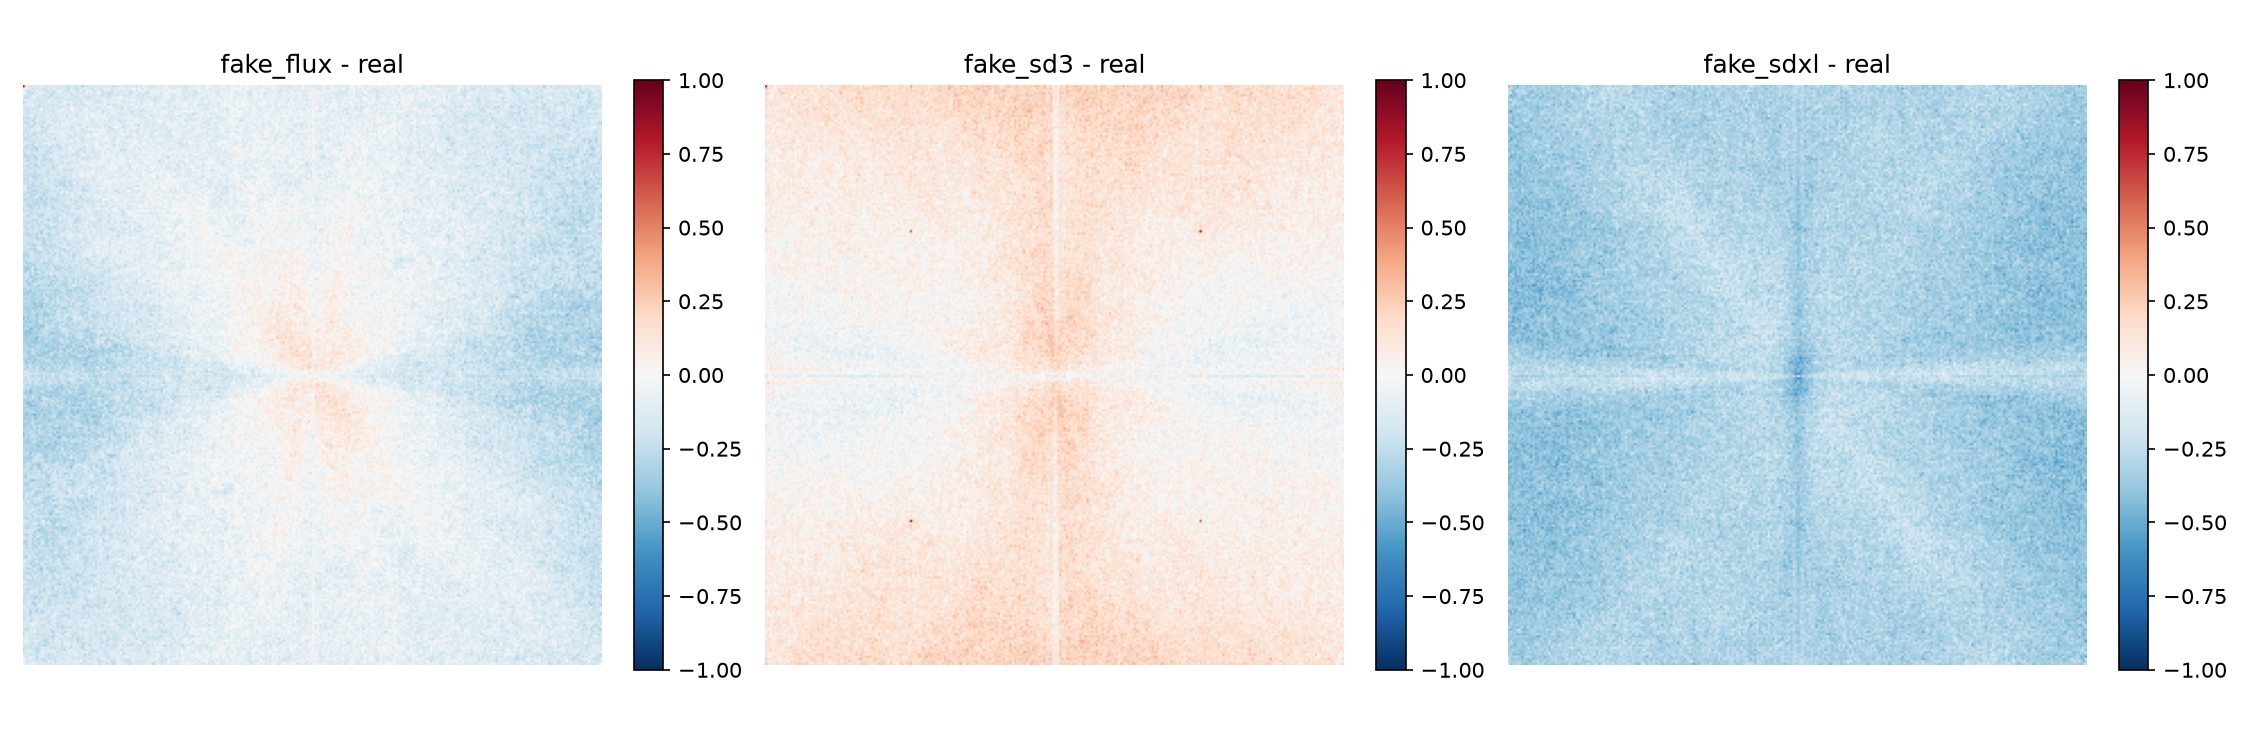
\includegraphics[width=\hsize]{figures/fig_spectra_diff.png}
\caption{Mean log-magnitude FFT difference from real images (fake minus
real), 300-image samples, for the three GenImage++ generators sharing one
real pool. Warm indicates more energy than real photographs at that
frequency, cool less. BigGAN and GLIDE are omitted because each is paired
with its own real split, so their maps are not comparable here.}
\label{fig:spectradiff}
\end{figure}

\subsection{Detectors fail by being confident, not uncertain}
\label{sec:confidence}

Figure~\ref{fig:scoredist} shows per-image predicted fake-probabilities for
UniversalFakeDetect. On FLUX.1 and SD3, where it fails hardest, the
fake-image distribution does not sit near the 0.5 boundary; it collapses
into the 0--0.1 bin, the region occupied by correctly classified real
images. On SDXL and GLIDE it retains visible mass near 1.0. The failure
mode is not borderline uncertainty but confident misclassification.

Reading that off a histogram is not enough, so we quantify it with expected
calibration error~\cite{guo2017calibration} over 15 equal-width bins
(Table~\ref{tab:auc}). The numbers track the failures:
UniversalFakeDetect's ECE is 0.042 on BigGAN, where it works, and 0.439 on
FLUX.1, where it does not, meaning average confidence overstates average
correctness by more than 43 points. A merely uncertain detector would push
scores toward 0.5 and produce a \emph{small} ECE alongside low accuracy;
instead accuracy falls and calibration error rises together, the signature
of confident error rather than abstention. The same holds for the CLIP
baseline on BigGAN (ECE 0.433 at 9.6\% fake-accuracy) and most starkly for
the ResNet-50 on BigGAN, whose ECE of 0.503 accompanies 0.4\%
fake-accuracy: wrong on essentially every generated image, and confident
about it. CLIP-LoRA is best-calibrated everywhere, never exceeding 0.020.

This matters for deployment. A detector that fails confidently gives a
downstream system no usable signal that it is outside its competence, and
thresholding, abstention and human-review routing all depend on low
confidence tracking low reliability.

\begin{figure}[t]
\centering
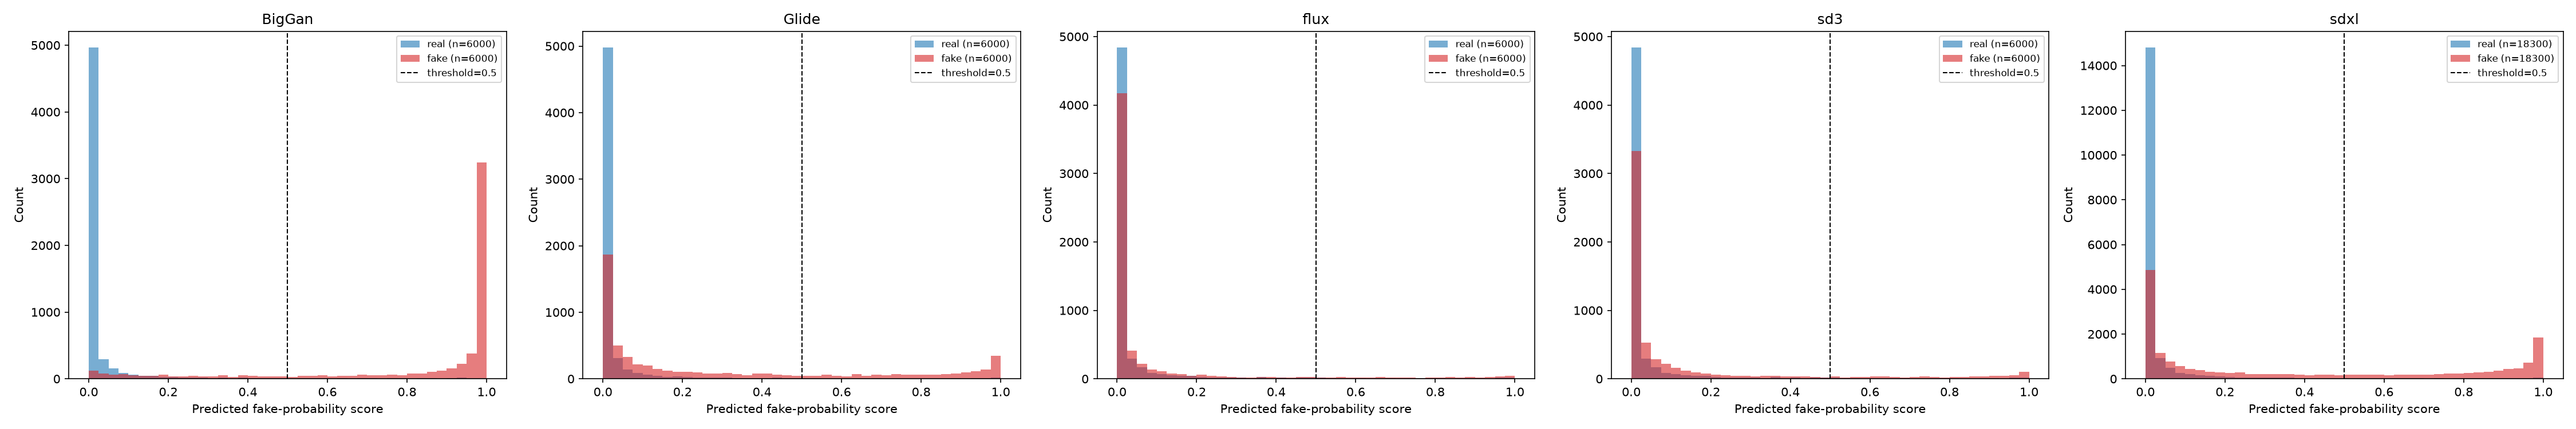
\includegraphics[width=\hsize]{figures/fig_score_dist_ufd.png}
\caption{UniversalFakeDetect predicted fake-probability scores, real (blue)
against fake (red), per generator. On FLUX.1 and SD3 the fake distribution
collapses into the same low-score region as real images; on BigGAN the
pattern mirrors in the opposite direction.}
\label{fig:scoredist}
\end{figure}

\section{Discussion: a preprocessing-driven reproducibility hazard}
\label{sec:discussion}

While preparing Table~\ref{tab:results}, our fake-accuracy for the
GenImage++ CLIP baseline on BigGAN (9.6\%) sat roughly 6x below the 62.66\%
the source paper reports for its own CLIP baseline on the same subset. A
disagreement of that size, on what should be the identical checkpoint and a
same-named benchmark, needed explaining before either number could be
trusted, so we treat the investigation as a contribution rather than a
footnote.

We first ruled out an implementation bug by reimplementing the source
repository's released \texttt{kornia}-based preprocessing and running both
versions over the same sixteen images through the same checkpoint. Scores
were near-identical, pointing at the preprocessing \emph{choice} rather
than a coding error.

GenImage's BigGAN subset ships fakes at 128$\times$128, unlike every other
generator in the benchmark (GLIDE ships at 256$\times$256), which is the
benchmark's documented convention rather than an artifact of our download.
The released preprocessing resizes every input to 224$\times$224 regardless
of native size, so BigGAN's fakes are upsampled nearly twofold while others
are downsampled or left near target. We added a second path preserving
native pixel scale, pasting onto a black canvas rather than interpolating,
and re-ran the full evaluation both ways for both checkpoints
(Table~\ref{tab:glidepreproc}, BigGAN rows). Padding moves the CLIP
baseline's overall accuracy to 61.66\%, within one point of the reported
62.66\%.

Two effects compound. The source paper's accuracy column is almost
certainly overall accuracy across both classes while our first measurement
was fake-only, a metric-definition mismatch on our end; and the resize
direction is a real effect we measured rather than inferred. The same swap
does the opposite to the OMAT checkpoint, dropping it from 99.7\% to
16.3\%, consistent with that paper's note that every fine-tuning strategy
used a fixed resize-to-224 pipeline.

We could not close the residual one point. GenImage's official
distribution is gated behind Baidu Yunpan and Google Drive with no
scriptable, authentication-free access, so we could not test against a
verified-authoritative sample, and the paper's own cross-benchmark
evaluation script is not among its released code. We report the limit
rather than assume the gap is fully explained.

\subsection{Does the effect generalize beyond BigGAN?}
\label{sec:glide-preproc}

An effect shown on one generator is an anecdote, so we repeated the test on
GLIDE, the only other generator here whose native resolution is not
224$\times$224. For the CLIP baseline it replicates in the same direction
at smaller magnitude: fake-accuracy 69.1\% to 76.9\% and AUC 94.0 to 97.4,
against 9.6\% to 25.3\% and AUC 68.0 to 90.4 on BigGAN. That ordering is
what the resolution gap predicts, GLIDE needing only a mild downsample
while BigGAN is upsampled twofold.

For CLIP-LoRA the two generators diverge completely. On GLIDE it is
unmoved (99.87\% to 99.77\%); on BigGAN it collapses (99.70\% to 16.28\%).
Inspecting the conditions explains why, and qualifies
Section~\ref{sec:finding2}. Our native-resolution path center-crops images
larger than 224 and zero-pads smaller ones. For GLIDE's 256$\times$256
inputs that is a pure center-crop with no border; for BigGAN's
128$\times$128 it produces a black frame covering 67.3\% of the canvas. The
two ``padding'' conditions are not the same operation, and the BigGAN
collapse is confounded between the absence of interpolation and the
presence of a large out-of-distribution border.

\begin{table}[h]
\caption{Padding versus official upsampling on the two generators whose
native resolution is not 224$\times$224, full evaluation sets. The GLIDE
padding condition is a pure center-crop; the BigGAN one introduces a black
border over 67.3\% of the canvas, so the two are not directly comparable.}
\label{tab:glidepreproc}
\begin{tabular*}{\hsize}{@{\extracolsep{\fill}}llrrr@{}}
\toprule
Generator & Checkpoint / preprocessing & Fake & Real & AUC \\
\colrule
BigGAN (128) & CLIP, upsample & 9.60 & 96.48 & 67.97 \\
BigGAN (128) & CLIP, padding & 25.30 & 98.02 & 90.38 \\
BigGAN (128) & CLIP-LoRA, upsample & 99.70 & 94.82 & 99.70 \\
BigGAN (128) & CLIP-LoRA, padding & 16.28 & 93.12 & 69.13 \\
GLIDE (256) & CLIP, upsample & 69.13 & 96.05 & 94.03 \\
GLIDE (256) & CLIP, padding & 76.93 & 98.20 & 97.44 \\
GLIDE (256) & CLIP-LoRA, upsample & 99.87 & 94.87 & 99.82 \\
GLIDE (256) & CLIP-LoRA, padding & 99.77 & 92.82 & 99.88 \\
\botrule
\end{tabular*}
\end{table}

\subsection{Separating interpolation from border artifacts}
\label{sec:disentangle}

We therefore ran a third condition on BigGAN: a nearest-neighbour upsample
to 224$\times$224, which removes smooth interpolation exactly as padding
does but introduces no border. On matched 2{,}000-image-per-class samples
the two causes separate cleanly.

Dropping interpolation alone costs CLIP-LoRA 37.8 points of fake-accuracy
(99.25\% to 61.45\%) while AUC falls only 1.7, from 99.63 to 97.90. An
accuracy collapse with ranking intact is a threshold problem: the model
still orders generated above real, but the score distribution has shifted
out from under the fixed cut. Adding the border is different damage.
Fake-accuracy falls to 5.30\% and AUC to 60.36, near enough to chance that
no threshold recovers it, so the border removes discriminative information
rather than relocating it.

This corrects Section~\ref{sec:finding2}. The BigGAN collapse is driven
mainly by the out-of-distribution border, not by the absence of
interpolation. The accurate statement is narrower: OMAT's hardening
survives a change of interpolation kernel in ranking terms while losing
threshold calibration, and fails outright only under a distortion with no
counterpart in its training pipeline, which is also why GLIDE, where no
border is introduced, leaves it untouched.

The CLIP baseline moves the opposite way on the same axis. Under
nearest-neighbour upsampling its AUC rises to 90.72 from 67.97 under the
official bicubic pipeline, so for a detector never fine-tuned against a
fixed pipeline, smooth interpolation of a 128$\times$128 output is itself
destroying signal. Two checkpoints trained on identical data prefer
opposite preprocessing, which is the sharpest form of the point: no
preprocessing choice is neutral across detectors, so a benchmark fixing one
implicitly favours some.

Together these support one claim: the same checkpoint, on the same images,
at the same threshold, yields materially different published-style accuracy
under defensible preprocessing conventions, and the direction is not
consistent even across checkpoints trained on identical data. Because
preprocessing is often under-specified in released code, and cross-generator
tables are routinely compared across papers applying their own conventions,
a reader comparing published numbers should treat a resize or crop mismatch
as a checkable explanation for an unexplained gap before concluding either
is wrong. The access barrier we hit also suggests a recommendation: a
benchmark intended for cross-paper comparison should ship a small,
scriptable, authentication-free verification subset, a few hundred images
with published checksums plus the exact preprocessing function and metric
definition behind its headline table. That requires neither redistributing
the dataset nor solving the hosting problem that pushes benchmarks onto
gated storage, and had one existed for GenImage this investigation would
have taken an afternoon rather than days.

\section{JPEG robustness, and a dataset bias it exposes}
\label{sec:robustness}

Images reaching a real detector have usually been re-encoded by whatever
platform carried them. We re-ran the FLUX.1 evaluation with every image
re-encoded at JPEG quality 75, holding the sample fixed at 2{,}000 per
class so the clean and compressed conditions are paired
(Table~\ref{tab:jpeg}).

\begin{table}[h]
\caption{FLUX.1 before and after JPEG quality-75 re-encoding (2{,}000 per
class, same sample in both conditions). NPR loses all discriminative
signal; the CLIP-family detectors lose accuracy but largely retain ranking.}
\label{tab:jpeg}
\begin{tabular*}{\hsize}{@{\extracolsep{\fill}}lcccc@{}}
\toprule
& \multicolumn{2}{c}{Fake-acc (\%)} & \multicolumn{2}{c}{AUC} \\
Detector & clean & JPEG-75 & clean & JPEG-75 \\
\colrule
UniversalFakeDetect & 7.30 & 6.00 & 61.19 & 55.54 \\
NPR & 98.00 & \textbf{1.50} & 97.10 & \textbf{50.63} \\
GenImage++ ResNet-50 & 69.45 & 58.00 & 91.27 & 88.48 \\
GenImage++ CLIP & 89.60 & 59.80 & 98.56 & 97.28 \\
GenImage++ CLIP-LoRA & 97.65 & 41.90 & 99.30 & 90.67 \\
\botrule
\end{tabular*}
\end{table}

NPR is the headline. It is the strongest detector on clean FLUX.1 by a wide
margin (98.0\%) and ordinary compression destroys it, falling to 1.50\%
with an AUC of 50.63, which is chance. This is mechanistically
unsurprising: NPR reads up-sampling artifacts in neighbouring-pixel
relationships, and JPEG quantisation attacks exactly the high-frequency
content those live in. The implication is sharp, since the detector a
clean-data leaderboard recommends is the one that fails most completely on
data that has passed through any normal image pipeline. The CLIP-family
detectors degrade more gracefully: the CLIP baseline loses 29.8 points of
fake-accuracy but only 1.3 of AUC, and CLIP-LoRA 55.8 against 8.6. An
accuracy drop far exceeding the AUC drop means the ranking still separates
the classes while the fixed threshold no longer sits in the right place,
which recalibration can fix; NPR's failure cannot be fixed that way,
because at an AUC of 50.6 no threshold helps.

\subsection{A compression confound in the underlying benchmarks}
\label{sec:jpeg-confound}

This also surfaced something that qualifies our absolute numbers, which we
report here rather than in a footnote. Across all five generators, every
generated image is distributed as PNG and every real image as JPEG: BigGAN
and GLIDE fakes are PNG at 128$\times$128 and 256$\times$256, GenImage++
fakes PNG at 1024$\times$1024, all reals ImageNet JPEGs. Real and generated
images therefore differ systematically in compression history, not only in
provenance, and a detector sensitive to compression artifacts can score
well by exploiting that.

The bias is documented for GenImage by Grommelt et
al.~\cite{grommelt2024jpeg}, who report that removing JPEG and
image-dimension confounds shifts cross-generator performance by more than
11 points. Our experiment estimates its size for the most
artifact-sensitive detector we test: once generated images carry JPEG
compression too, NPR's ability to separate the classes vanishes. We cannot
conclude that NPR's clean 98.0\% is \emph{entirely} a compression artifact,
since JPEG re-encoding also destroys genuine generative traces and both
explanations predict the same collapse. But NPR's clean FLUX.1 result
should not be read as a pure measurement of generative-artifact detection,
and every absolute accuracy on these benchmarks carries the confound.

Two things limit the damage. All five detectors saw exactly the same
images, so the cross-detector comparisons and every paired test in
Section~\ref{sec:significance} remain valid even if absolute levels are
inflated by a shared bias. And the confound is a property of the real/fake
pairing, so it cannot explain Section~\ref{sec:finding-shape}, where two
detectors on identical images produce identical difficulty orderings at
very different levels. Repeating this study on a compression-balanced
benchmark, such as the debiased GenImage variant released
with~\cite{grommelt2024jpeg}, is the most important single follow-up.

\section{Limitations}
\label{sec:limitations}

Detector diversity is narrower than ``five detectors'' suggests: three
share a CLIP backbone family. The two convolutional detectors are
structurally distinct from that family and from each other in training
data, which is why we lean on them when separating architecture from
training distribution. Findings holding across all five are on firmer
ground than those from the CLIP family alone. A genuinely independent
family, such as a diffusion-reconstruction method~\cite{wang2023dire}, is
the most valuable single addition future work could make.

Cross-detector real-accuracy on FLUX.1, SD3 and SDXL is unpaired: because
GenImage++ ships no reals, each run drew its own sample from the shared
162{,}000-image pool and those sets overlap only incidentally (7 of
6{,}000 for FLUX.1 and SD3, 200 of 18{,}300 for SDXL). The fake sets are
identical across all five detectors for every generator, so fake-accuracy
comparisons and every paired test are properly paired; BigGAN and GLIDE are
matched on both classes. Separately, whether the ImageNet images behind the
GenImage++ checkpoints' training subset overlap our real pools is
unresolved from released materials; it would not affect the fake-accuracy
findings but could slightly inflate real-accuracy for those checkpoints.
Their exact training composition rests on the source paper's own reported
methodology, which we could not check against training logs.

All detectors run at a fixed 0.5 threshold with no tuning, so the accuracy
figures are out-of-the-box behaviour rather than each detector's best
operating point, which is why AUC is reported alongside. On cost, since we
motivate the study partly by deployment: the three CLIP detectors run at
7.4--7.6 images per second (132--139~ms each) on our 8~GB GPU, while NPR
runs at 229--320 per second, roughly 35 times faster. That is not
incidental, since NPR is both the cheapest detector here and the strongest
on the two Diffusion Transformers, so the detector chosen on throughput is
not the one chosen from headline accuracy. We report throughput rather than
isolated latency because batch inference is the realistic deployment mode.

\section{Conclusion}
\label{sec:conclusion}

Five pretrained detectors, evaluated on five generators with leakage
verified absent, disagree about which generator is hardest, and the
disagreement is statistically real rather than sampling noise. What
predicts a detector's weak spot is its training distribution, not the
generator's recency: BigGAN, the oldest generator here, is the hardest case
for two detectors and among the easiest for two others.

Adding a detector trained on the same data as an existing one but on a
different architecture sharpens that into something more useful than
``training data matters.'' The two rank the five generators identically
while differing 37.6 points in mean accuracy. On the evidence here,
training distribution appears to fix the shape of a failure profile and the
representation its level, which would mean a stronger backbone raises
accuracy without moving the blind spot. That is a two-detector observation
and we mark it as such, but it is testable, and it predicts that ensembling
detectors chosen for different \emph{training lineages} should beat
ensembling for architectural variety.

The failure mode is what makes these gaps consequential. Calibration error
rises alongside error rate rather than falling, so a detector leaving its
training distribution does not signal its own unreliability through lower
confidence; it stays confident and becomes wrong. Adversarial training on
on-manifold latent perturbations closes most of the accuracy gap and yields
the best-calibrated detector we test, the most encouraging result here, and
its robustness proved more durable than our first reading suggested,
surviving a change of interpolation kernel and failing only under a
distortion with no counterpart in its training pipeline.

Two findings temper how any of these numbers should be used. Ordinary JPEG
re-encoding takes NPR from the best FLUX.1 detector we measure to
chance-level AUC, so the detector a clean-data leaderboard recommends is
the one least suited to deployment. And in every benchmark we use,
generated images are PNG while real images are JPEG, a compression
asymmetry documented by prior work~\cite{grommelt2024jpeg} that can account
for a large share of one detector's apparent skill. Cross-detector
comparisons survive this, since every detector saw the same images, but
absolute accuracies should be treated as upper bounds. The investigation
behind that caveat began as an unexplained 6x gap against a published
number and ended in a metric-definition mismatch plus a real preprocessing
effect. Until benchmarks ship the small verification subsets we recommend
in Section~\ref{sec:discussion}, cross-paper accuracy comparisons in this
literature should be read with that possibility in mind.

\section{Ethical and dual-use considerations}
\label{sec:ethics}

Documenting where detectors fail is dual-use: the table telling a platform
which detector to avoid also tells an evader which generator to prefer. We
think publication is still right. The detectors and generators are already
public, so these failure modes are discoverable by anyone willing to run
the same inference; nothing here is a new capability. The information
asymmetry currently runs against defenders, who often deploy a single
detector assuming a published number transfers, which our results show it
does not. And our concrete recommendations, combining detectors with
different training lineages and reporting calibration and preprocessing
alongside accuracy, are defensive rather than evasive.

Two narrower cautions. None of these detectors should be sole evidence in a
consequential decision about a person, given that the best-calibrated one
still misclassifies a meaningful fraction of real images and the worst is
confidently wrong most of the time on some generators. And our results are
measured on ImageNet-derived object and scene imagery; we make no claim
about images of people, and face manipulation is out of scope entirely.

\section*{Acknowledgements}

\appendix
\section{Data and code availability}
Detector checkpoints and evaluation datasets used in this study are the
original authors' public releases, cited in Table~\ref{tab:detectors} and
Section~\ref{sec:methods}. The evaluation harness, the per-image prediction
scores for every detector and generator reported here, the paired
significance tests, the calibration computations, and the
preprocessing-sensitivity analysis of Section~\ref{sec:discussion} will be
released publicly upon publication; the repository link is withheld here
only to preserve review anonymity and will be inserted in the
camera-ready version.

\begin{thebibliography}{99}

\bibitem{wang2020cnndetect}
Wang, Sheng-Yu, Oliver Wang, Richard Zhang, Andrew Owens, and Alexei A.\ Efros.
(2020) ``CNN-generated images are surprisingly easy to spot... for now.''
\textit{Proceedings of the IEEE/CVF Conference on Computer Vision and
Pattern Recognition}: 8695--8704.

\bibitem{genimage2023}
Zhu, Mingjian, Hanting Chen, Qiangyu Yan, Xudong Huang, Guanyu Lin, Wei Li,
Zhijun Tu, Hailin Hu, Jie Hu, and Yunhe Wang. (2023) ``GenImage: A
million-scale benchmark for detecting AI-generated image.''
\textit{Advances in Neural Information Processing Systems} \textbf{36}:
77771--77782.

\bibitem{ojha2023universal}
Ojha, Utkarsh, Yuheng Li, and Yong Jae Lee. (2023) ``Towards Universal Fake
Image Detectors that Generalize Across Generative Models.''
\textit{Proceedings of the IEEE/CVF Conference on Computer Vision and
Pattern Recognition}: 24480--24489.

\bibitem{tan2024npr}
Tan, Chuangchuang, Yao Zhao, Shikui Wei, Guanghua Gu, Ping Liu, and Yunchao
Wei. (2024) ``Rethinking the Up-Sampling Operations in CNN-based
Generative Network for Generalizable Deepfake Detection.''
\textit{Proceedings of the IEEE/CVF Conference on Computer Vision and
Pattern Recognition}: 28130--28139.

\bibitem{zhou2025omat}
Zhou, Yue, Xinan He, KaiQing Lin, Bin Fan, Feng Ding, and Bin Li. (2025)
``Breaking Latent Prior Bias in Detectors for Generalizable AIGC Image
Detection.'' \textit{arXiv preprint arXiv:2506.00874}.

\bibitem{flux2024}
Black Forest Labs. (2024) ``FLUX.'' \url{https://github.com/black-forest-labs/flux}.

\bibitem{esser2024sd3}
Esser, Patrick, Sumith Kulal, Andreas Blattmann, Rahim Entezari, Jonas
M\"{u}ller, Harry Saini, Yam Levi, Dominik Lorenz, Axel Sauer, Frederic
Boesel, et al. (2024) ``Scaling rectified flow transformers for
high-resolution image synthesis.'' \textit{Forty-first International
Conference on Machine Learning}.

\bibitem{brock2019biggan}
Brock, Andrew, Jeff Donahue, and Karen Simonyan. (2019) ``Large scale GAN
training for high fidelity natural image synthesis.'' \textit{International
Conference on Learning Representations}.

\bibitem{nichol2021glide}
Nichol, Alex, Prafulla Dhariwal, Aditya Ramesh, Pranav Shyam, Pamela
Mishkin, Bob McGrew, Ilya Sutskever, and Mark Chen. (2021) ``GLIDE:
Towards photorealistic image generation and editing with text-guided
diffusion models.'' \textit{arXiv preprint arXiv:2112.10741}.

\bibitem{podell2023sdxl}
Podell, Dustin, Zion English, Kyle Lacey, Andreas Blattmann, Tim Dockhorn,
Jonas M\"{u}ller, Joe Penna, and Robin Rombach. (2023) ``SDXL: Improving
latent diffusion models for high-resolution image synthesis.''
\textit{arXiv preprint arXiv:2307.01952}.

\bibitem{radford2021clip}
Radford, Alec, Jong Wook Kim, Chris Hallacy, Aditya Ramesh, Gabriel Goh,
Sandhini Agarwal, Girish Sastry, Amanda Askell, Pamela Mishkin, Jack Clark,
et al.\ (2021) ``Learning transferable visual models from natural language
supervision.'' \textit{International Conference on Machine Learning}:
8748--8763.

\bibitem{hu2022lora}
Hu, Edward J., Yelong Shen, Phillip Wallis, Zeyuan Allen-Zhu, Yuanzhi Li,
Shean Wang, Lu Wang, and Weizhu Chen. (2022) ``LoRA: Low-rank adaptation of
large language models.'' \textit{International Conference on Learning
Representations}.


\bibitem{peebles2023dit}
Peebles, William, and Saining Xie. (2023) ``Scalable diffusion models with
transformers.'' \textit{Proceedings of the IEEE/CVF International
Conference on Computer Vision}: 4195--4205.


\bibitem{xu2025seeds}
Xu, Katherine, Lingzhi Zhang, and Jianbo Shi. (2025) ``Good seed makes
good crop: Discovering secret seeds in text-to-image diffusion models.''
\textit{IEEE/CVF Winter Conference on Applications of Computer Vision}:
3024--3034.

\bibitem{wang2023dire}
Wang, Zhendong, Jianmin Bao, Wengang Zhou, Weilun Wang, Hezhen Hu, Hong
Chen, and Houqiang Li. (2023) ``DIRE for diffusion-generated image
detection.'' \textit{Proceedings of the IEEE/CVF International Conference
on Computer Vision}: 22445--22455.

\bibitem{yan2024chameleon}
Yan, Shilin, Ouxiang Li, Jiayin Cai, Yanbin Hao, Xiaolong Jiang, Yao Hu,
and Weidi Xie. (2024) ``A sanity check for AI-generated image detection.''
\textit{arXiv preprint arXiv:2406.19435}.

\bibitem{qian2020freq}
Qian, Yuyang, Guojun Yin, Lu Sheng, Zixuan Chen, and Jing Shao. (2020)
``Thinking in frequency: Face forgery detection by mining
frequency-aware clues.'' \textit{European Conference on Computer Vision}:
86--103.

\bibitem{tan2025c2pclip}
Tan, Chuangchuang, Renshuai Tao, Huan Liu, Guanghua Gu, Baoyuan Wu, Yao
Zhao, and Yunchao Wei. (2025) ``C2P-CLIP: Injecting category common
prompt in CLIP to enhance generalization in deepfake detection.''
\textit{Proceedings of the AAAI Conference on Artificial Intelligence}
\textbf{39}: 7184--7192.

\bibitem{rossler2019ff}
R\"{o}ssler, Andreas, Davide Cozzolino, Luisa Verdoliva, Christian Riess,
Justus Thies, and Matthias Nie{\ss}ner. (2019) ``FaceForensics++: Learning
to detect manipulated facial images.'' \textit{Proceedings of the IEEE/CVF
International Conference on Computer Vision}: 1--11.

\bibitem{li2020celebdf}
Li, Yuezun, Xin Yang, Pu Sun, Honggang Qi, and Siwei Lyu. (2020)
``Celeb-DF: A large-scale challenging dataset for deepfake forensics.''
\textit{Proceedings of the IEEE/CVF Conference on Computer Vision and
Pattern Recognition}: 3207--3216.


\bibitem{frank2020leveraging}
Frank, Joel, Thorsten Eisenhofer, Lea Sch\"{o}nherr, Asja Fischer, Dorothea
Kolossa, and Thorsten Holz. (2020) ``Leveraging frequency analysis for deep
fake image recognition.'' \textit{International Conference on Machine
Learning}: 3247--3258.

\bibitem{selvaraju2017gradcam}
Selvaraju, Ramprasaath R., Michael Cogswell, Abhishek Das, Ramakrishna
Vedantam, Devi Parikh, and Dhruv Batra. (2017) ``Grad-CAM: Visual
explanations from deep networks via gradient-based localization.''
\textit{Proceedings of the IEEE International Conference on Computer
Vision}: 618--626.

\bibitem{guo2017calibration}
Guo, Chuan, Geoff Pleiss, Yu Sun, and Kilian Q. Weinberger. (2017) ``On
calibration of modern neural networks.'' \textit{International Conference
on Machine Learning}: 1321--1330.

\bibitem{mcnemar1947}
McNemar, Quinn. (1947) ``Note on the sampling error of the difference
between correlated proportions or percentages.'' \textit{Psychometrika}
\textbf{12} (2): 153--157.

\bibitem{grommelt2024jpeg}
Grommelt, Patrick, Louis Weiss, Franz-Josef Pfreundt, and Janis Keuper.
(2024) ``Fake or JPEG? Revealing common biases in generated image detection
datasets.'' \textit{arXiv preprint arXiv:2403.17608}.

\end{thebibliography}

\end{document}
